\documentclass{file/KP-ITS}

\newtheorem{defn}{Definisi}[section]
\newtheorem{teo}[defn]{Teorema}
\newtheorem{thm}{Teorema}[section]
\newtheorem{lemma}[defn]{Lemma}
\newtheorem{lemmas}[thm]{Lemma}
\newtheorem{cor}[defn]{Akibat}
\theoremstyle{definition}
\newtheorem{con}[defn]{Contoh}
\theoremstyle{definition}
\theoremstyle{plain}
\newtheorem{prop}[defn]{Proposisi}
\renewcommand{\proofname}{Bukti}
\renewcommand{\thethm}{\arabic{chapter}.\arabic{thm}}

\newcommand{\norm}[1]{\left\|#1\right\|} % Fungsi norm (||x||)

\newcommand\firstPar{0.75cm} % Indentasi 0.75cm pada tiap paragraf (manual untuk hspace)
\setlength{\parindent}{0.75cm} % Indentasi 0.75cm pada tiap paragraf

\usepackage{fancyhdr}
\pagestyle{fancy}
\renewcommand{\headrulewidth}{0pt}
\fancyhf{}
\fancyfoot[R]{\thepage}

\usepackage[labelsep=quad]{caption}
% \captionsetup[table]{skip=5pt}

\usepackage{multirow}
\usepackage{longtable}


%%% Pewarnaan code
\usepackage{color}
\usepackage{listings}
\usepackage[outline]{contour}

\definecolor{codegreen}{rgb}{0,0.6,0}
\definecolor{codeblack}{rgb}{0,0,0}
\definecolor{codepurple}{rgb}{0.58,0,0.82}
\definecolor{backcolour}{rgb}{0.95,0.95,0.92}

\lstdefinestyle{mystyle}{
    commentstyle=\color{codegreen},
    keywordstyle=\color{magenta},
    numberstyle=\tiny\color{codeblack},
    stringstyle=\color{codepurple},
    basicstyle=\ttfamily\footnotesize,
    breakatwhitespace=false,         
    breaklines=true,                 
    captionpos=b,                    
    keepspaces=true,                 
    numbers=left,                    
    numbersep=5pt,                  
    showspaces=false,                
    showstringspaces=false,
    showtabs=false,                  
    tabsize=2
}

\usepackage{minted}
\setminted[js]{fontsize=\scriptsize,frame=lines,framesep=2mm,linenos=true,breaklines=true,breakanywhere=true,}
\setminted[css]{fontsize=\scriptsize,frame=lines,framesep=2mm,linenos=true,breaklines=true,breakanywhere=true,bgcolor=backcolour,}

%%% Pewarnaan code

\usepackage{hyperref}
\hypersetup{ % Merubah warna link
    colorlinks,
    linkcolor={black},
    citecolor={black},
    urlcolor={black}
}
\usepackage{tikz}
\usetikzlibrary{shapes, arrows.meta, positioning}

\definecolor{ioColor}{HTML}{D4E1F5}
\definecolor{processColor}{HTML}{FFE599}
\definecolor{decisionColor}{HTML}{FFCE9F}

\tikzstyle{startstop} = [rectangle, rounded corners, 
minimum width=2cm, 
minimum height=1cm,
text centered, 
draw=black, 
fill=pink]

\tikzstyle{io} = [trapezium, 
trapezium stretches=true, 
trapezium left angle=70, 
trapezium right angle=110, 
minimum width=2cm, 
minimum height=1cm, text centered, 
draw=black,text centered, 
text width=2.5cm,fill=ioColor]

\tikzstyle{process} = [rectangle, 
minimum width=2cm, 
minimum height=1cm, 
text centered, 
text width=2.5cm, 
draw=black,fill=processColor]

\tikzstyle{decision} = [diamond, 
minimum width=2cm, 
minimum height=1cm, 
text centered, 
draw=black,fill=decisionColor]

\tikzstyle{arrow} = [text width=2cm,thick, ->, >=stealth]

\tikzstyle{sumjunction} = [draw,
    circle,
    minimum size=0.7cm,
    text centered,
    path picture={
      \draw [black] % atau pakai warna lain yang pasti ada
        (path picture bounding box.135) -- (path picture bounding box.315)
        (path picture bounding box.45) -- (path picture bounding box.225);
    }
]

\begin{document}

% input data
\NamaPerusahaan{Subdirektorat Koordinasi Perkuliahan Bersama}

\Judul{Perancangan Website Interaktif untuk Pembelajaran Kalkulus Menggunakan CortexJS}

\JudulEng{Design of an Interactive Website for Calculus Learning Using CortexJS}

\Nama{Teosofi Hidayah Agung}

\NamaKecil{Teosofi Hidayah Agung}

\NRP{5002221132}

\Departemen{Matematika}

\Department{Mathematics}

\BidangStudi{Aljabar dan Analisis}

\AlamatPenulis{Jalan Kendangsari Gang VII/22, RT.06 RW.03, Surabaya}

\Bulan{Mei} % Masuk lembar pengesahan

\Tahun{2025}

\TanggalDisetujui{31 Mei 2025} % Masuk lembar orisinilitas

\Fakultas{Sains dan Analitika Data}

\SingkatanFakultas{FSAD}

\Faculty{Scientics}

\SingkatanFakultasEng{SCIENTICS}

\Pembimbing{Dr. Didik Khusnul A, S.Si, M.Si}
          {} 	   

\NIPPembimbing{197309301997021001}
{} 
              
\Kadep{Dr. Didik Khusnul A, S.Si, M.Si}

\NIPKadep{197309301997021001}

\PembimbingMitra{Refais Akbar Zufira, S.Kom}

\NIPPembimbingMitra{1998202121057}

\KepalaInstansi{Dr. Bintoro Anang S, S.Si., M.Si.}

\JabatanKepalaInstansi{Kepala Subdirektorat Koordinasi \\Perkuliahan Bersama}

\NIPKepalaInstansi{197907192005011015}
\BagianAwal
\Cover
\LembarJudul
\TitlePage
\LembarPengesahanDepartemen
\LembarPengesahanInstansi
\LembarOrisinalitas

%%%%%%%%%%%%%%%%%%%%%%%%  Kata Pengantar %%%%%%%%%%%%%%%5%%%%%%%%%%
\restoregeometry
\KataPengantar
Puji syukur penulis panjatkan kehadirat Allah SWT, Tuhan Yang Maha Esa, atas segala rahmat dan karunia-Nya sehingga penulis dapat menyelesaikan laporan Kerja Praktik ini dengan baik. Laporan ini disusun sebagai salah satu syarat untuk menyelesaikan mata kuliah Kerja Praktik di Departemen Matematika, Institut Teknologi Sepuluh Nopember (ITS).

%%%%%%%%%%%%%%%%%%%%%%%%  Daftar  %%%%%%%%%%%%%%%5%%%%%%%%%%

\DaftarIsi

\DaftarGambar

\DaftarTabel

% \DaftarSimbol
% \begin{flushleft}
% \begin{tabular}{lrl}


% $\oplus$ &:& Operasi \textit{max} dalam aljabar max-plus\\

% \end{tabular}
% \end{flushleft}
%%%%%%%%%%%%%%%%%%%%%%%%  Daftar  %%%%%%%%%%%%%%%5%%%%%%%%%%

\BagianInti

%%%%%%%%%%%%%%%%%%%%%%%%  Bab I  %%%%%%%%%%%%%%%5%%%%%%%%%%
\chapter{PENDAHULUAN}
\section{Latar Belakang}
Perkembangan teknologi informasi yang semakin pesat telah mendorong perubahan signifikan dalam berbagai aspek kehidupan, termasuk di dunia pendidikan. Dalam menghadapi tantangan tersebut, diperlukan keterlibatan langsung mahasiswa di lapangan untuk memahami bagaimana teknologi dapat dimanfaatkan secara nyata dalam proses pembelajaran \cite{suryadi2019}. Oleh karena itu, mahasiswa tidak hanya dituntut untuk menguasai teori di bangku kuliah, tetapi juga perlu memiliki pengalaman praktik dalam mengembangkan solusi berbasis teknologi yang aplikatif dan relevan dengan kebutuhan saat ini.

Kerja Praktik merupakan salah satu mata kuliah wajib yang harus ditempuh oleh seluruh mahasiswa Departemen Matematika, Institut Teknologi Sepuluh Nopember (ITS), sebagai bagian dari kurikulum pendidikan sarjana. Mata kuliah ini memberikan kesempatan bagi mahasiswa untuk mengaplikasikan ilmu yang telah diperoleh selama masa perkuliahan ke dalam dunia kerja yang nyata. Selain itu, kerja praktik juga bertujuan untuk melatih kemampuan problem solving, komunikasi, kolaborasi, serta kedisiplinan mahasiswa dalam lingkungan kerja profesional.

Pada kerja praktik ini, penulis mendapatkan kesempatan untuk melaksanakan program kerja di salah satu subdirektorat kampus ITS yang bergerak dalam bidang pengembangan teknologi informasi dan pembelajaran digital. Proyek utama yang diamanahkan kepada penulis adalah merancang dan mengembangkan sebuah \textit{website} pembelajaran interaktif untuk mata kuliah Kalkulus, yang merupakan mata kuliah dasar dan sangat fundamental bagi mahasiswa jurusan sains dan teknik.

Kalkulus sering kali menjadi tantangan tersendiri bagi mahasiswa, terutama dalam memahami konsep abstrak dan penerapan rumus-rumus matematis. Oleh karena itu, dibutuhkan sebuah media pembelajaran alternatif yang menarik, interaktif, dan mudah diakses guna membantu mahasiswa memahami materi dengan lebih efektif. Pemanfaatan teknologi web menjadi solusi yang relevan, mengingat mayoritas aktivitas akademik saat ini telah bergeser ke platform digital \cite{mustafidah2010,rahmawati2018}.

Melalui kerja praktik ini, penulis tidak hanya berkontribusi dalam pembangunan sistem berbasis web, tetapi juga memperluas wawasan tentang penerapan matematika dalam dunia nyata, terutama dalam bidang pengembangan teknologi pendidikan. Diharapkan proyek ini dapat memberikan manfaat jangka panjang bagi mahasiswa ITS, khususnya dalam meningkatkan kualitas pembelajaran Kalkulus secara mandiri dan fleksibel.

\section{Tujuan Kerja Praktik}
Dalam penulisan laporan Kerja Praktik ini mempunyai tujuan umum dan tujuan khusus sebagai berikut:
\subsection{Tujuan Umum}
Tujuan umum Kerja Praktik adalah sebagai berikut:
\begin{itemize}
    \item Memenuhi salah satu mata kuliah wajib di Departemen Matematika ITS untuk tahap sarjana.
    \item Menerapkan ilmu yang diperoleh di perkuliahan dalam dunia kerja.
    \item Memperoleh pengalaman bekerja di bawah bimbingan seorang pembimbing di tempat Kerja Praktik.
\end{itemize}

\subsection{Tujuan Khusus}
Tujuan khusus Kerja Praktik adalah sebagai berikut:
\begin{itemize}
    \item Mengimplementasikan ide \textit{project website} interaktif untuk pembelajaran kalkulus menggunakan \textit{framework} CortexJS.
    \item Menambah wawasan dan pengalaman dalam dunia \textit{web development}.
\end{itemize}

\section{Manfaat}
Berisikan manfaat yang diperoleh dari tujuan umum maupun
%%%%%%%%%%%%%%%%%%%%%%%%  Bab I  %%%%%%%%%%%%%%%5%%%%%%%%%%

%%%%%%%%%%%%%%%%%%%%%%%%  Bab II  %%%%%%%%%%%%%%%5%%%%%%%%%%

\pagebreak
\chapter{GAMBARAN UMUM SKPB}

\section{Sejarah SKPB}
Subdirektorat Koordinasi Perkuliahan Bersama (SKPB) adalah unit di bawah Direktorat Pendidikan yang bertanggung jawab untuk mengatur perkuliahan mata kuliah bersama bagi semua mahasiswa di ITS. Direktorat Pendidikan dibentuk berdasarkan Peraturan Rektor ITS No. 24 Tahun 2019 mengenai Organisasi dan Tata Kerja ITS yang diimplementasikan pada tahun 2020. Direktorat Pendidikan merupakan hasil penggabungan dari unit-unit sebelumnya, yaitu Biro Administrasi Pembelajaran dan Kemahasiswaan (BAPKM) serta Direktorat Akademik yang berfungsi dari tahun 2016 sampai 2020. Biro Administrasi Pembelajaran dan Kesejahteraan Mahasiswa mengelola semua tahapan administrasi pendidikan untuk mahasiswa yang dipimpin oleh Kepala Biro. Sementara itu, Direktorat Akademik memiliki tanggung jawab dalam merumuskan kebijakan akademik termasuk kurikulum dan dipimpin oleh seorang Direktur. Pada tahun itu, tidak ada pemisahan antara lembaga pelayanan untuk program sarjana dan pascasarjana. 

Pada tahun sebelumnya, yakni 2014-2016, lembaga administrasi Pendidikan ini dikenal sebagai Biro Akademik, Kemahasiswaan, dan Perencanaan (BAKP), hasil penggabungan dari Badan Akademik yang didirikan antara tahun 2012 hingga 2014 dan dipimpin oleh Kepala Badan. Lebih dulu lagi, lembaga ini sebelumnya dikenal sebagai Biro Administrasi Akademik dan Kemahasiswaan (BAAK)
\section{Struktur Organisasi}
SKPB berada di bawah Direktorat Pengembangan Akademik dan Inovasi Pembelajaran (DPAIP) yang berada pada bidang 1 yang dimana berkoordinasi dengan Wakil Rektor 1 Bidang Akademik dan Kemahasiswaan. Berikut adalah struktur organisasi Direktorat Pengembangan Akademik dan Inovasi Pembelajaran (DPAIP) yang mengelola SKPB:
\begin{figure}[h!]
    \centering
    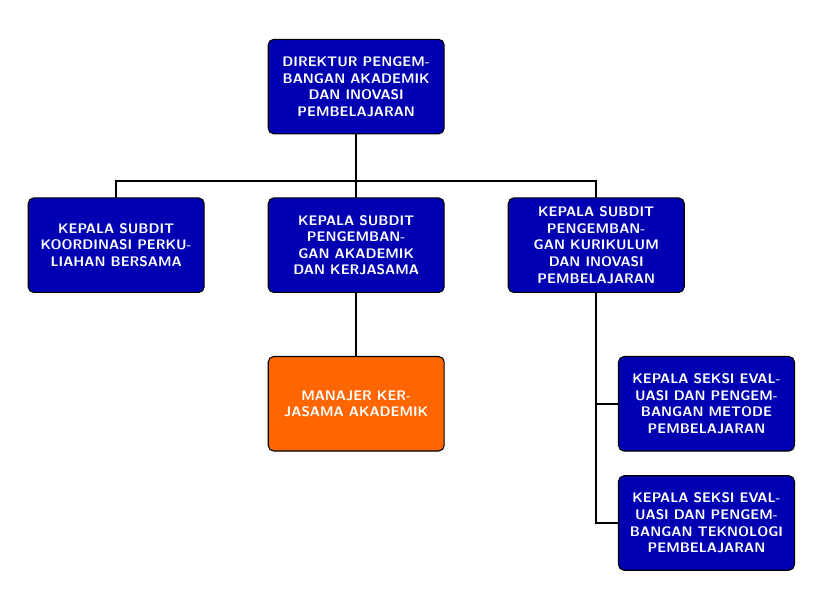
\begin{tikzpicture}[
    node distance=0.8cm and 0.8cm,
    dosen/.style={draw=black,rectangle, rounded corners=2pt, minimum width=2cm, minimum height=1.2cm, align=center, text=white, fill=blue!70!black, font=\bfseries\sffamily\tiny, text width=2cm},
    tendik/.style={draw=black,rectangle, rounded corners=2pt, minimum width=2cm, minimum height=1.2cm, align=center, text=white, fill=orange!80!red, font=\bfseries\sffamily\tiny, text width=2cm},
    line/.style={draw, thick,line cap=rect}
]

% Root
\node[dosen] (root) {DIREKTUR PENGEMBANGAN AKADEMIK DAN INOVASI PEMBELAJARAN};
\node[draw=none, above=of root, yshift=-0.9cm] (empty) {};

% Level 1
\node[dosen, below left=of root,] (d1) {KEPALA SUBDIT KOORDINASI PERKULIAHAN BERSAMA};
\node[dosen, below=of root] (d2) {KEPALA SUBDIT PENGEMBANGAN AKADEMIK DAN KERJASAMA};
\node[dosen, below right=of root,] (d3) {KEPALA SUBDIT PENGEMBANGAN KURIKULUM DAN INOVASI PEMBELAJARAN};

% Tendik bawah d2
\node[tendik, below=of d2] (t1) {MANAJER KERJASAMA AKADEMIK};

% Tendik bawah d3
\node[dosen, below=of d3,xshift=1.4cm] (d4) {KEPALA SEKSI EVALUASI DAN PENGEMBANGAN METODE PEMBELAJARAN};
\node[dosen, below=of d4,yshift=0.5cm] (d5) {KEPALA SEKSI EVALUASI DAN PENGEMBANGAN TEKNOLOGI PEMBELAJARAN};

% Draw lines
\draw[line] (root) |-++(0,-1.2) -| (d1);
\draw[line] (root) -- (d2);
\draw[line] (root) |-++(0,-1.2) -| (d3);
\draw[line] (d2) -- (t1);
\draw[line] (d3) |- (d4);
\draw[line] (d3) |- (d5);
\end{tikzpicture}
    \caption{Struktur Organisasi DPAIP}
    \label{fig:struktur-organisasi-dpaip}
\end{figure}

\section{Kegiatan Perusahaan}
Berdasarkan Pasal 8 Peraturan Rektor ITS No. 26 Tahun 2019, tugas dan fungsi Subdirektorat Koordinasi Perkuliahan Bersama dapat diuraikan sebagai berikut:
\begin{enumerate}
    \item Subdirektorat Koordinasi Perkuliahan Bersama mempunyai tugas membantu Direktorat Pendidikan dalam:
    \begin{enumerate}
        \item Membantu merumuskan kebijakan dalam lingkup koordinasi perkuliahan bersama.
        \item Membina, mengarahkan dan mengembangkan kompetensi dan talenta personil dalam unit kerja.
        \item Menyelenggarakan program kerja dan kegiatan yang selaras dengan kebijakan dalam lingkup koordinasi perkuliahan bersama.
        \item Mengevaluasi kinerja hasil program kerja dan kegiatan dalam lingkup koordinasi perkuliahan bersama.
        \item Menyelenggarakan layanan prima dalam lingkup koordinasi perkuliahan bersama dengan prinsip reformasi birokrasi dan zona integritas.
    \end{enumerate}

    \item Dalam melaksanakan tugas sebagaimana dimaksud pada poin (1), Subdirektorat Koordinasi Perkuliahan Bersama menyelenggarakan fungsi:
    \begin{enumerate}
        \item Pengkajian dan penyelenggaraan mata kuliah wajib nasional dan mata kuliah ITS untuk program sarjana dan vokasi.
        \item Pengkajian dan pengembangan kuliah bersama untuk program sarjana dan vokasi dengan prinsip kolaborasi dan \textit{sharing} sumber daya.
        \item Penyelenggaraan kuliah bersama untuk program sarjana dan vokasi.
        \item Pengawasan dan evaluasi penyelenggaraan mata kuliah wajib nasional, mata kuliah ITS, dan kuliah bersama untuk program sarjana dan vokasi.
        \item Koordinasi dan fasilitasi penyelenggaraan kuliah lintas perguruan tinggi.
    \end{enumerate}
\end{enumerate}


% (\ref*{pers1}). % Merujuk persamaan tinggal menuliskan labelnya


%%%%%%%%%%%%%%%%%%%%%%%%  Bab II  %%%%%%%%%%%%%%%5%%%%%%%%%%

%%%%%%%%%%%%%%%%%%%%%%%%  Bab III  %%%%%%%%%%%%%%%5%%%%%%%%%%

\pagebreak
\chapter{PELAKSANAAN KERJA PRAKTIK}

\section{Pelaksanaan Kerja Praktik}
Berikut adalah keterangan pelaksanaan kerja praktik yang sudah dilakukan selama sekitar 2 bulan:
% \vspace*{-0.5cm}
\begin{flushleft}
\begin{tabular}{lcp{0.7\textwidth}}
    Waktu	&:& 16 Desember 2024 - 9 Februari 2025 \\
    Tempat &:& Subdirektorat Koordinasi Perkuliahan Bersama (SKPB) ITS
\end{tabular}
\end{flushleft}
\noindent Perihal keterangan rangkaian kerja praktik selengkapnya dilampirkan pada Lampiran.

\section{Metodologi Penyelesaian Tugas Khusus}
Berikut merupakan metodologi penyelesaian dalam bentuk diagram alir:
\begin{figure}[h!]
\centering
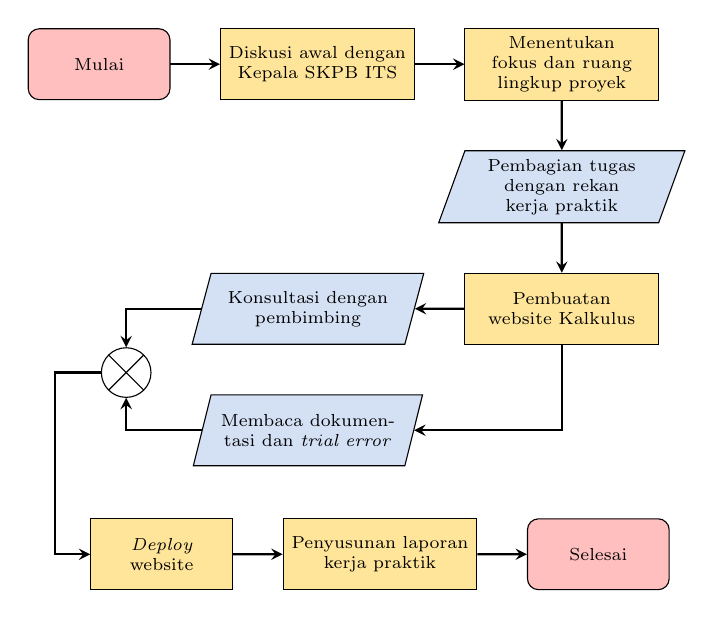
\begin{tikzpicture}[node distance=0.7cm and 0.7cm,font=\scriptsize,scale=0.9,transform shape]
    % Nodes
    \node[startstop] (start) {Mulai};
    \node[process, right=of start] (diskusi) {Diskusi awal dengan Kepala SKPB ITS};
    \node[process, right=of diskusi] (ruanglingkup) {Menentukan fokus dan ruang lingkup proyek};
    \node[io, below=of ruanglingkup] (pembagian) {Pembagian tugas dengan rekan kerja praktik};
    \node[process, below=of pembagian] (pembuatan) {Pembuatan website Kalkulus};
    \node[io, left=of pembuatan] (bimbingan) {Konsultasi dengan pembimbing};
    \node[io, below=of bimbingan] (studi) {Membaca dokumentasi dan \textit{trial error}};
    \node[sumjunction, left=of bimbingan,yshift=-0.9cm] (sum) {};
    \node[process, below=of sum,text width=1.5cm,xshift=0.5cm,yshift=-1cm] (upload) {\textit{Deploy} website};
    \node[process, right=of upload] (laporan) {Penyusunan laporan kerja praktik};
    \node[startstop, right=of laporan] (end) {Selesai};

    % Arrows
    \draw[arrow] (start) -- (diskusi);
    \draw[arrow] (diskusi) -- (ruanglingkup);
    \draw[arrow] (ruanglingkup) -- (pembagian);
    \draw[arrow] (pembagian) -- (pembuatan);
    \draw[arrow] (pembuatan) -- (bimbingan);
    \draw[arrow] (pembuatan) |- (studi);
    \draw[arrow] (bimbingan) -| (sum);
    \draw[arrow] (studi) -| (sum);
    \draw[arrow] (sum) -| ++(-1,0) |- (upload);
    \draw[arrow] (upload) -- (laporan);
    \draw[arrow] (laporan) -- (end);
\end{tikzpicture}
\caption{Alur Kegiatan Kerja Praktik di SKPB ITS}
\end{figure}
\begin{enumerate}
    \item Melakukan diskusi awal dengan Kepala SKPB ITS untuk memahami permasalahan yang sedang dihadapi dalam mendukung pembelajaran matematika dasar di lingkungan ITS.
    \item Menentukan fokus permasalahan yang akan diselesaikan melalui kerja praktik serta mendefinisikan ruang lingkup proyek.
    \item Membagi tugas dan tanggung jawab bersama rekan kerja praktik.
    \item Merancang dan mengembangkan media pembelajaran berupa website interaktif untuk mata kuliah Kalkulus 1 dan Kalkulus 2.
    \item Melakukan konsultasi rutin dengan pembimbing lapangan dari SKPB ITS untuk mengevaluasi kemajuan serta mendapatkan masukan.
    \item Melakukan studi referensi dengan membaca dokumentasi dan menonton tutorial sebagai panduan dalam proses pengembangan website pembelajaran.
    \item Menyusun laporan kerja praktik berdasarkan proses perencanaan, pelaksanaan, dan hasil yang telah dicapai selama kegiatan.
    \item Mempresentasikan hasil kerja praktik kepada SKPB ITS dan dosen pembimbing sebagai bentuk pertanggungjawaban dan evaluasi akhir.
\end{enumerate}

\subsection{HTML}

HTML (HyperText Markup Language) merupakan bahasa markah yang digunakan untuk membangun struktur dasar halaman web. HTML mendefinisikan elemen-elemen seperti judul, paragraf, tautan, dan tabel, yang kemudian diterjemahkan oleh peramban menjadi tampilan visual halaman web. Elemen-elemen ini diatur dengan tag yang menyatakan struktur logis dari konten web. HTML menjadi dasar penting dalam pengembangan website karena menentukan hierarki dan susunan konten yang akan ditampilkan \cite{sharma2024}.

\subsection{CSS}

CSS (Cascading Style Sheets) adalah bahasa yang digunakan untuk mengatur presentasi dari dokumen yang ditulis dalam HTML. CSS memungkinkan pemisahan antara konten dan desain, sehingga pengembang dapat mengubah tampilan situs web (warna, font, tata letak) tanpa mengubah struktur HTML-nya. Penggunaan CSS yang efektif dapat meningkatkan aksesibilitas dan estetika situs, serta memudahkan pemeliharaan dan pengembangan web secara berkelanjutan \cite{hasan2022}.

\subsection{JavaScript}

JavaScript merupakan bahasa pemrograman yang berperan penting dalam pengembangan website interaktif dan dinamis. Dalam konteks pendidikan, JavaScript memungkinkan pembuatan media pembelajaran yang lebih menarik dan responsif, sehingga dapat meningkatkan keterlibatan mahasiswa dalam proses belajar. Penggunaan JavaScript dalam pengembangan website pembelajaran telah terbukti efektif dalam meningkatkan kualitas interaksi pengguna dan penyampaian materi \cite{insana2021pengembangan}.

\subsection{CortexJS}

CortexJS adalah pustaka JavaScript yang dirancang untuk mempermudah manipulasi dan visualisasi ekspresi matematika di web. Dengan CortexJS, pengembang dapat menyajikan notasi matematika secara interaktif, yang sangat berguna dalam pembuatan konten pembelajaran kalkulus dan mata pelajaran matematika lainnya. Dokumentasi resmi CortexJS menyediakan berbagai fitur yang mendukung pembuatan konten matematika yang dinamis dan user-friendly \cite{cortexjs2025}.

\subsection{Github}

GitHub adalah platform yang menyediakan layanan hosting untuk pengembangan perangkat lunak berbasis Git. Dalam pengembangan website pembelajaran, GitHub memfasilitasi kolaborasi antar tim pengembang, manajemen versi kode, serta integrasi dan pengujian berkelanjutan. Penggunaan GitHub dalam konteks pendidikan juga telah diterapkan sebagai media e-learning yang efektif, memungkinkan siswa untuk belajar langsung melalui proyek nyata dan meningkatkan keterampilan pemrograman mereka \cite{rahmawati2021penerapan}.

%%%%%%%%%%%%%%%%%%%%%%%%  Bab III  %%%%%%%%%%%%%%%5%%%%%%%%%%

\chapter{HASIL KERJA PRAKTIK}
\section{Komponen dalam Website}

Banyaknya komponen dalam website yang dibuat menjadikan tim pengembang harus bekerja sama dan berbagai tugas agar website dapat selesai tepat waktu. Penulis mendapatkan tugas untuk membuat beberapa komponen website, diantaranya sebagai berikut dapat dilihat pada gambar di bawah ini
\begin{figure}[h!]
    \centering
    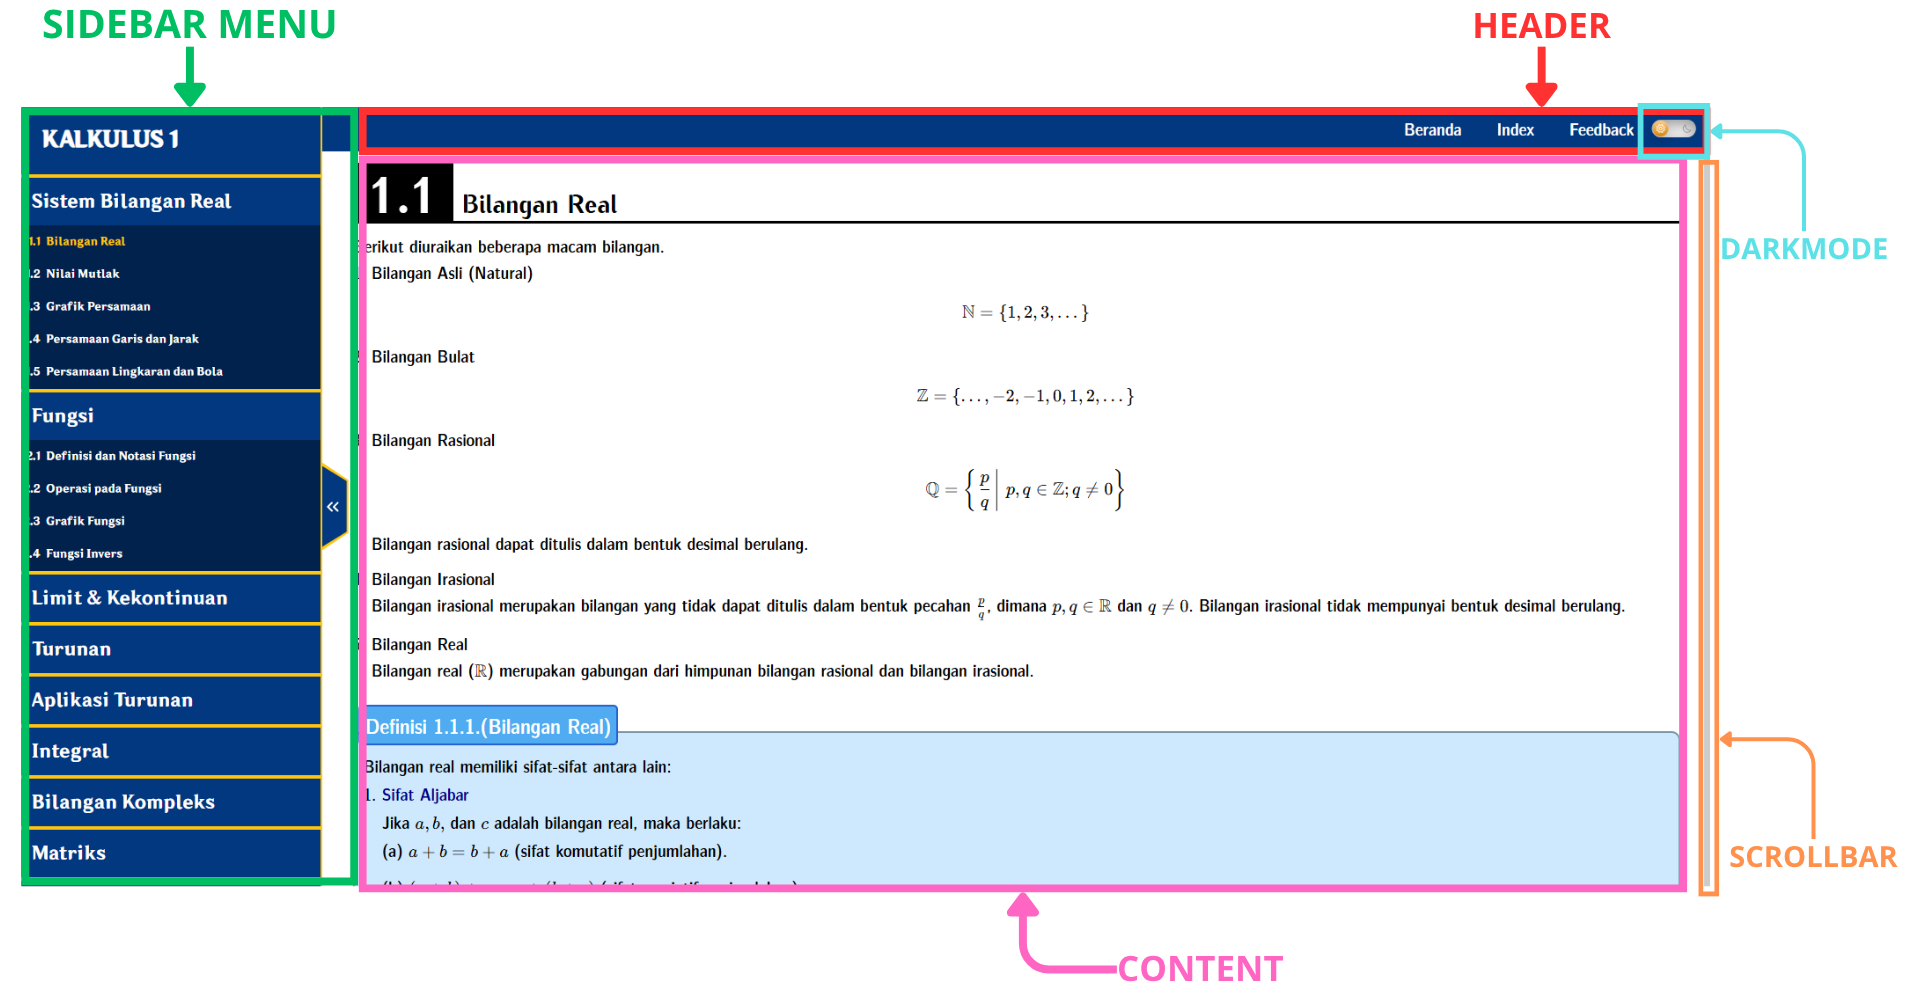
\includegraphics[width=\textwidth]{foto/KomponenWeb.png}
    \caption{Komponen dalam Website Pembelajaran Interaktif}
\end{figure}\\
Setiap komponen memiliki fungsi dan tujuan masing-masing sehingga mereka dibungkus (\textit{encapsulated}) dalam \textit{tag} HTML yang sesuai. 

\subsection{\textit{Header}}
\textit{Header} adalah bagian atas dari halaman web yang berisi tombol untuk menuju Beranda, index materi, dan pengisian feedback bagi pengguna. Selain itu \textit{header} juga terdapat bagian \textit{toggle} untuk mengaktifkan atau menonaktifkan \textit{darkmode} pada website.

\subsection{\textit{Darkmode}}
\textit{Darkmode} adalah fitur yang memungkinkan pengguna untuk mengubah tema tampilan website menjadi gelap. Fitur ini dirancang untuk mengurangi ketegangan mata saat melihat layar dalam kondisi pencahayaan rendah. Pengguna dapat dengan mudah mengaktifkan atau menonaktifkan \textit{darkmode} melalui tombol yang tersedia di \textit{header}.
\begin{figure}[h!]
    \centering
    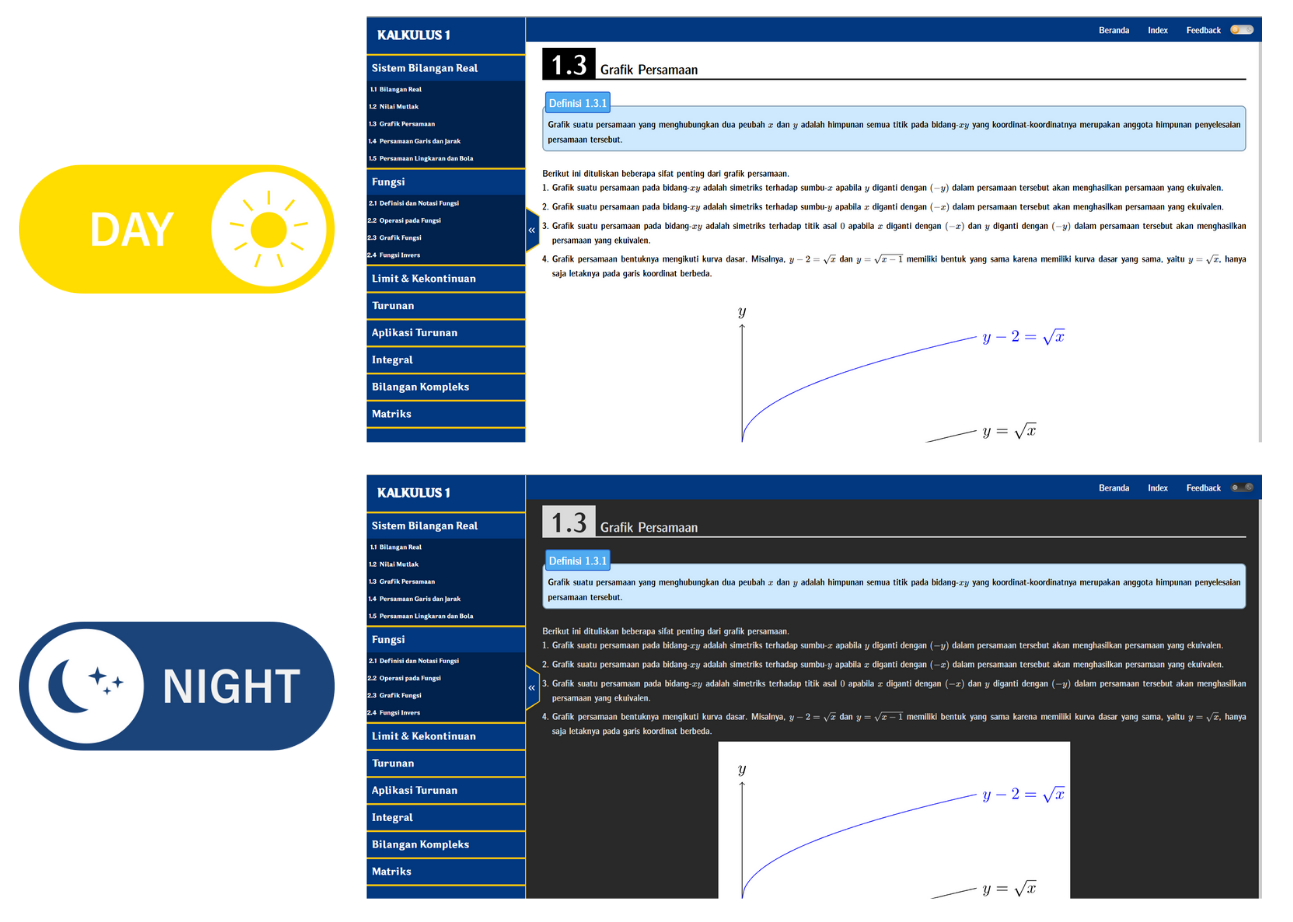
\includegraphics[width=\textwidth]{foto/LightDarkMode.png}
    \caption{Perbedaan Tampilan Website Fitur Darkmode}
\end{figure}
\subsection{\textit{Sidebar Menu}}
Sidebar menu adalah komponen penting dalam website yang berfungsi sebagai navigasi utama. Komponen ini memungkinkan pengguna untuk dengan mudah mengakses berbagai bagian dari website, seperti materi pembelajaran dan tombol kembali ke beranda. Berikut adalah kode CSS yang digunakan untuk mengatur tampilan sidebar menu:

\begin{minted}{css}
.sidebar{
  box-sizing: border-box;
  font-family: HYWenHei;
  width: fit-content;
  position: sticky;
  align-self: start;
  overflow: hidden;
  ... /* Properti lainnya */
}
\end{minted}
Dalam kode di atas, properti CSS \texttt{position: sticky} digunakan untuk menjaga posisi sidebar tetap terlihat saat pengguna menggulir halaman. Selain itu, properti \texttt{overflow: hidden} memastikan bahwa konten yang melebihi batas sidebar tidak akan terlihat, sehingga menjaga tampilan tetap rapi.
\begin{figure}[h!]
    \centering
    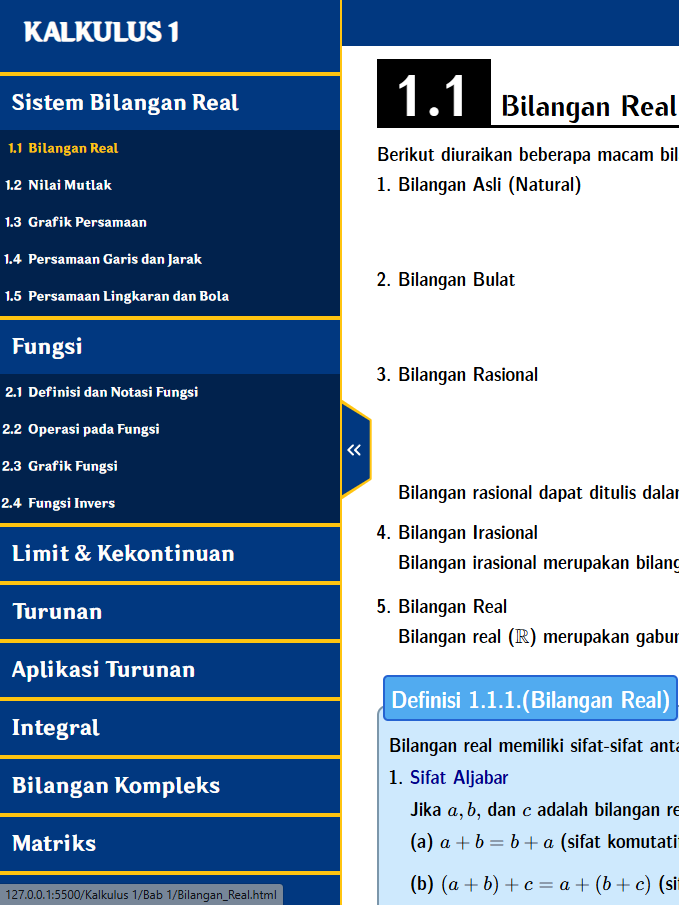
\includegraphics[width=0.4\textwidth]{foto/SidebarBuka.png}$\qquad$
    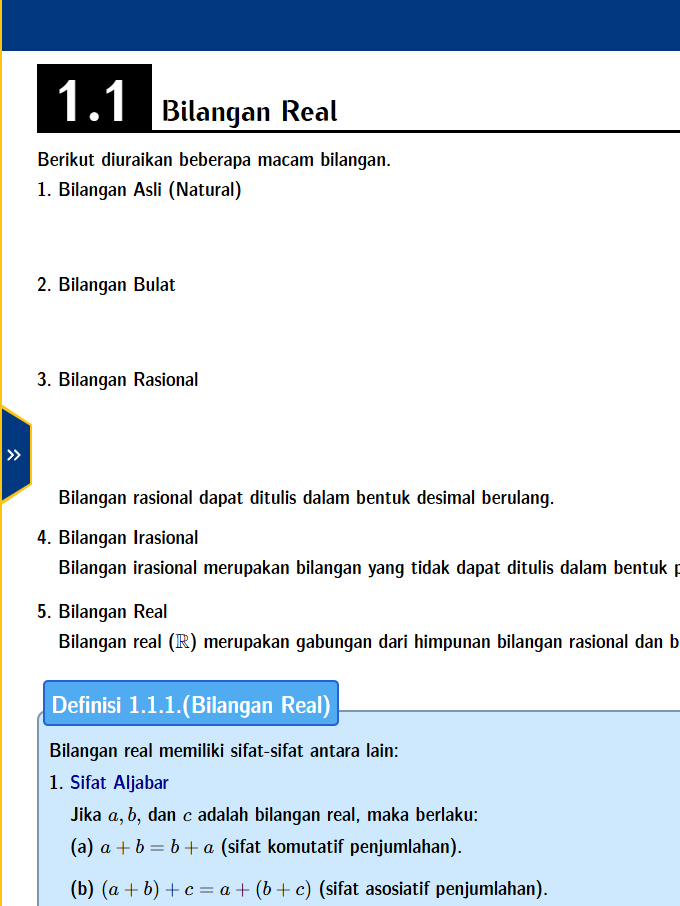
\includegraphics[width=0.4\textwidth]{foto/SidebarTutup.png}
    \caption{Tampilan Sidebar Menu saat Terbuka dan Tertutup}
\end{figure}

\subsection{Latihan \textit{Box}}

\subsection{\textit{Math-Field}}

\section{Implementasi CortexJS dalam interaktivitas Website}

%%%%%%%%%%%%%%%%%%%%%%%%  Bab IV %%%%%%%%%%%%%%%5%%%%%%%%%%

\chapter{PENUTUP}
\section{Kesimpulan}
Berdasarkan hasil kerja praktik yang telah dilakukan, dapat disimpulkan bahwa:
\begin{enumerate}
    \item 
\end{enumerate}
\section{Saran}

%%%%%%%%%%%%%%%%%%%%%%%%  Bab V %%%%%%%%%%%%%%%5%%%%%%%%%%


\DaftarPustaka
%%%%%%%%%%%%%%%%%%%%%%%%  Dapus  %%%%%%%%%%%%%%%5%%%%%%%%%%

\cleardoublepage
\lampiran{\textit{Logbook} Kegiatan}
\begin{longtable}{|c|>{\centering\arraybackslash}p{0.31\linewidth}|>{\raggedright\arraybackslash}p{0.5\linewidth}|}
    \caption{Jadwal Kegiatan Kerja Praktik} \\
    \hline
    \rowcolor{gray!30}\textbf{No} & \textbf{Tanggal} & \centering\arraybackslash\textbf{Deskripsi Kegiatan} \\
    \hline
    \endfirsthead

    \multicolumn{3}{c}%
    {{ \thetable{} -- lanjutan dari halaman sebelumnya}} \\
    \hline
    \rowcolor{gray!30}\textbf{No} & \textbf{Tanggal} & \centering\arraybackslash\textbf{Deskripsi Kegiatan} \\
    \hline
    \endhead

    1 & 16 Desember 2024 (08.00 - 16.30 WIB) & Mengenal lingkungan kerja \\
    \hline
    2 & 17 Desember 2024 (11.00 - 16.00 WIB) & Berdiskusi tujuan KP dari masing-masing individu \\
    \hline
    3 & 18 Desember 2024 (12.00 - 16.00 WIB) & Belajar dasar website HTML CSS \\
    \hline
    4 & 19 Desember 2024 (12.00 - 16.00 WIB) & Fiksasi jobdesk masing-masing individu \\
    \hline
    5 & 23 Desember 2024 (10.00 - 16.00 WIB) & Lanjutan belajar web HTML CSS Javascript \\
    \hline
    6 & 6 Januari 2025 (11.00 - 16.00 WIB) & Mulai membuat tampilan awal web \\
    \hline
    7 & 7 Januari 2025 (12.00 - 16.00 WIB) & Menonton dan mengimplementasikan template web dari YouTube \\
    \hline
    8 & 8 Januari 2025 (13.00 - 16.00 WIB) & Membuat sidebar menu \\
    \hline
    9 & 9 Januari 2025 (14.00 - 16.00 WIB) & Mencari referensi tentang \textbf{CoretexJS} sebagai penunjang interaktivitas web \\
    \hline
    10 & 13 Januari 2025 (13.00 - 16.00 WIB) & Mempelajari fitur-fitur CSS Wrapped 2024 \\
    \hline
    11 & 14 Januari 2025 (13.00 - 16.00 WIB) & Mengimplementasikan fitur CSS Wrapped 2024 ke dalam prototype website \\
    \hline
    12 & 16 Januari 2025 (14.00 - 16.00 WIB) & Mulai menginputkan materi sambil membuat template CSS komponen yang lain \\
    \hline
    13 & 17 Januari 2025 (13:00 - 16:00 WIB) & Menemukan referensi untuk komponen \textit{Definition box} \\
    \hline
    14 & 20 Januari 2025 (9:30 - 16:00 WIB) & Mencoba \textbf{CortexJS} ke dalam website \\
    \hline
    15 & 21 Januari 2025 (12:00 - 16:00 WIB) & Mengoptimalkan animasi serta responsif \texttt{math-field} \\
    \hline
    16 & 23 Januari 2025 (12:00 - 16:00 WIB) & Belajar meng-\textit{convert} gambar tikz menjadi svg menggunakan \texttt{dvisvgm} \\
    \hline
    17 & 30 Januari 2025 (11:00 - 16:00 WIB) & Mengoptimalkan CSS \\
    \hline
    18 & 3 Februari 2025 (11:00 - 16:00 WIB) & Mengoptimalkan sidebar menu \\
    \hline
    19 & 4 Februari 2025 (11:00 - 16:00 WIB) & Mengoptimalkan tabel dalam web \\
    \hline
    20 & 5 Februari 2025 (10:00 - 16:00 WIB) & Mempresentasikan hasil ke pembimbing \\
    \hline
    21 & 6 Februari 2025 (11:00 - 16:00 WIB) & Membuat \textit{Hint Box} \\
    \hline
    22 & 7 Februari 2025 (13:30 - 16:00 WIB) & Melanjutkan menginput materi ke file HTML \\
    \hline
\end{longtable}

\cleardoublepage
\lampiran{Kode Script CortexJS}
\begin{minted}{js}
import "//unpkg.com/mathlive?module";
import "//unpkg.com/@cortex-js/compute-engine";

const ce = MathfieldElement.computeEngine;

const answerButton = document.getElementById("submitAnswer");
const answerElements = document.querySelectorAll(".answer");

const bgColorAnswer = answerElements[0].style.backgroundColor;
const borderColorAnswer = answerElements[0].style.borderColor;

const correctAnswers = [
  ce.parse("\\left\\lbrace x\\le\\frac94\\right\\rbrace"),
  ce.parse("\\left\\lbrace x>\\frac13\\right\\rbrace"),
];

answerButton.addEventListener("click", () => {
  answerElements.forEach((answerElement) => {
    answerElement.style.backgroundColor = bgColorAnswer;
    answerElement.style.borderColor = borderColorAnswer;
  });
  answerElements.forEach((answerElement, index) => {
    let studentInput = answerElement.expression;
    const expectedAnswer = correctAnswers[index];
  if (
    index == 0 &&
    (answerElement.value ===
      "\\left(-\\infty,\\frac94\\right\\rbrack" ||
      answerElement.value === "(-\\infty,\\frac94\\rbrack" ||
      answerElement.value === "\\left(-\\infty,\\9/4\\right\\rbrack" ||
      answerElement.value === "(-\\infty,\\9/4\\rbrack")
  ) {
    studentInput = expectedAnswer;
  }
    if (
      studentInput.isSame(ce.parse("\\left(\\frac13,+\\infty\\right)"))
    ) {
      studentInput = expectedAnswer;
    }
    const loading = document.getElementById("loading");
    const feedback = document.querySelectorAll(".jawaban-latihan");
    loading.classList.remove("hidden");
  setTimeout(() => {
    loading.classList.add("hidden");
    feedback.forEach((el) => {
      el.classList.remove("hidden");
    });
    if (!studentInput.isSame(expectedAnswer)) {
      answerElement.style.backgroundColor = "rgba(255, 192, 203, 0.5)";
      answerElement.style.borderColor = "red";
    } else {
      answerElement.style.backgroundColor = "rgba(172, 255, 47, 0.5)";
      answerElement.style.borderColor = "green";
    }
  }, 2000);
 });
});
\end{minted}
%%%%%%%%%%%%%%%%%%%%%%%%  Lampiran %%%%%%%%%%%%%%%5%%%%%%%%%%

\cleardoublepage
\Biodata{foto/FotoPenulis}
\textbf{Teosofi Hidayah Agung}, lahir di Surabaya pada 8 Juni 2025. Penulis merupakan mahasiswa aktif Departemen Matematika, Institut Teknologi Sepuluh Nopember (ITS) Surabaya angkatan 2022. Lahir dari keluarga sederhana beranggotakan ayah, ibu, nenek, dan kakak perempuan bersama-sama tinggal di Kota Pahlawan. Penulis menyelesaikan pendidikan dasar di SDN Iskandar Said Surabaya pada tahun 2017, kemudian melanjutkan pendidikan menengah di SMPN 35 Surabaya hingga tahun 2020, dan melanjutkan pendidikan menengah atas di MAN Surabaya sebagai siswa kelas Akselerasi yang lulus pada tahun 2022. 
%%%%%%%%%%%%%%%%%%%%%%%%  Bio Penulis  %%%%%%%%%%%%%%%5%%%%%%%%%%
\end{document}